\subsection{Trasmissione di segnali}

In questa parte dell'esperienza ci occuperemo di effettuare la trasmissione di segnali attraverso un circuito logico. Ovviamente potremmo dedicare ad ogni segnale un filo: dunque, se volessimo trasportare $N$ segnali dovremmo utilizzare $N$ fili.

Un modo più efficiente è segnalare a chi deve ricevere il segnale quale di questi $N$ segnali stia passando su un unico cavo di trasmissione. Dobbiamo quindi predisporre una circuiteria dedicata al \textit{segnale di selezione} e dovremmo portare tanti cavi quanti siano necessari ad identificare univocamente tutti gli $N$ segnali.

Ad esempio, nel nostro caso abbiamo bisogno di mandare quattro segnali distinti, quindi avremo bisogno di due segnali di selezione (infatti le combinazioni di 1 e 0 logici possibili sono abbastanza per assegnare ad ognuno dei quattro segnali un codice logico di due cifre). Dunque, insieme al cavo dedicato alla trasmissione dati e a quello di terra (abbiamo bisogno di un riferimento comune per i nostri stati logici), costruiremo un circuito di trasmissione che utilizzerà quattro cavi e avrà bisogno di blocchi per la selezione e blocchi per la trasmissione.

\subsubsection{Selettore}

\begin{wrapfigure}[10]{l}{0.45\textwidth}
\centering
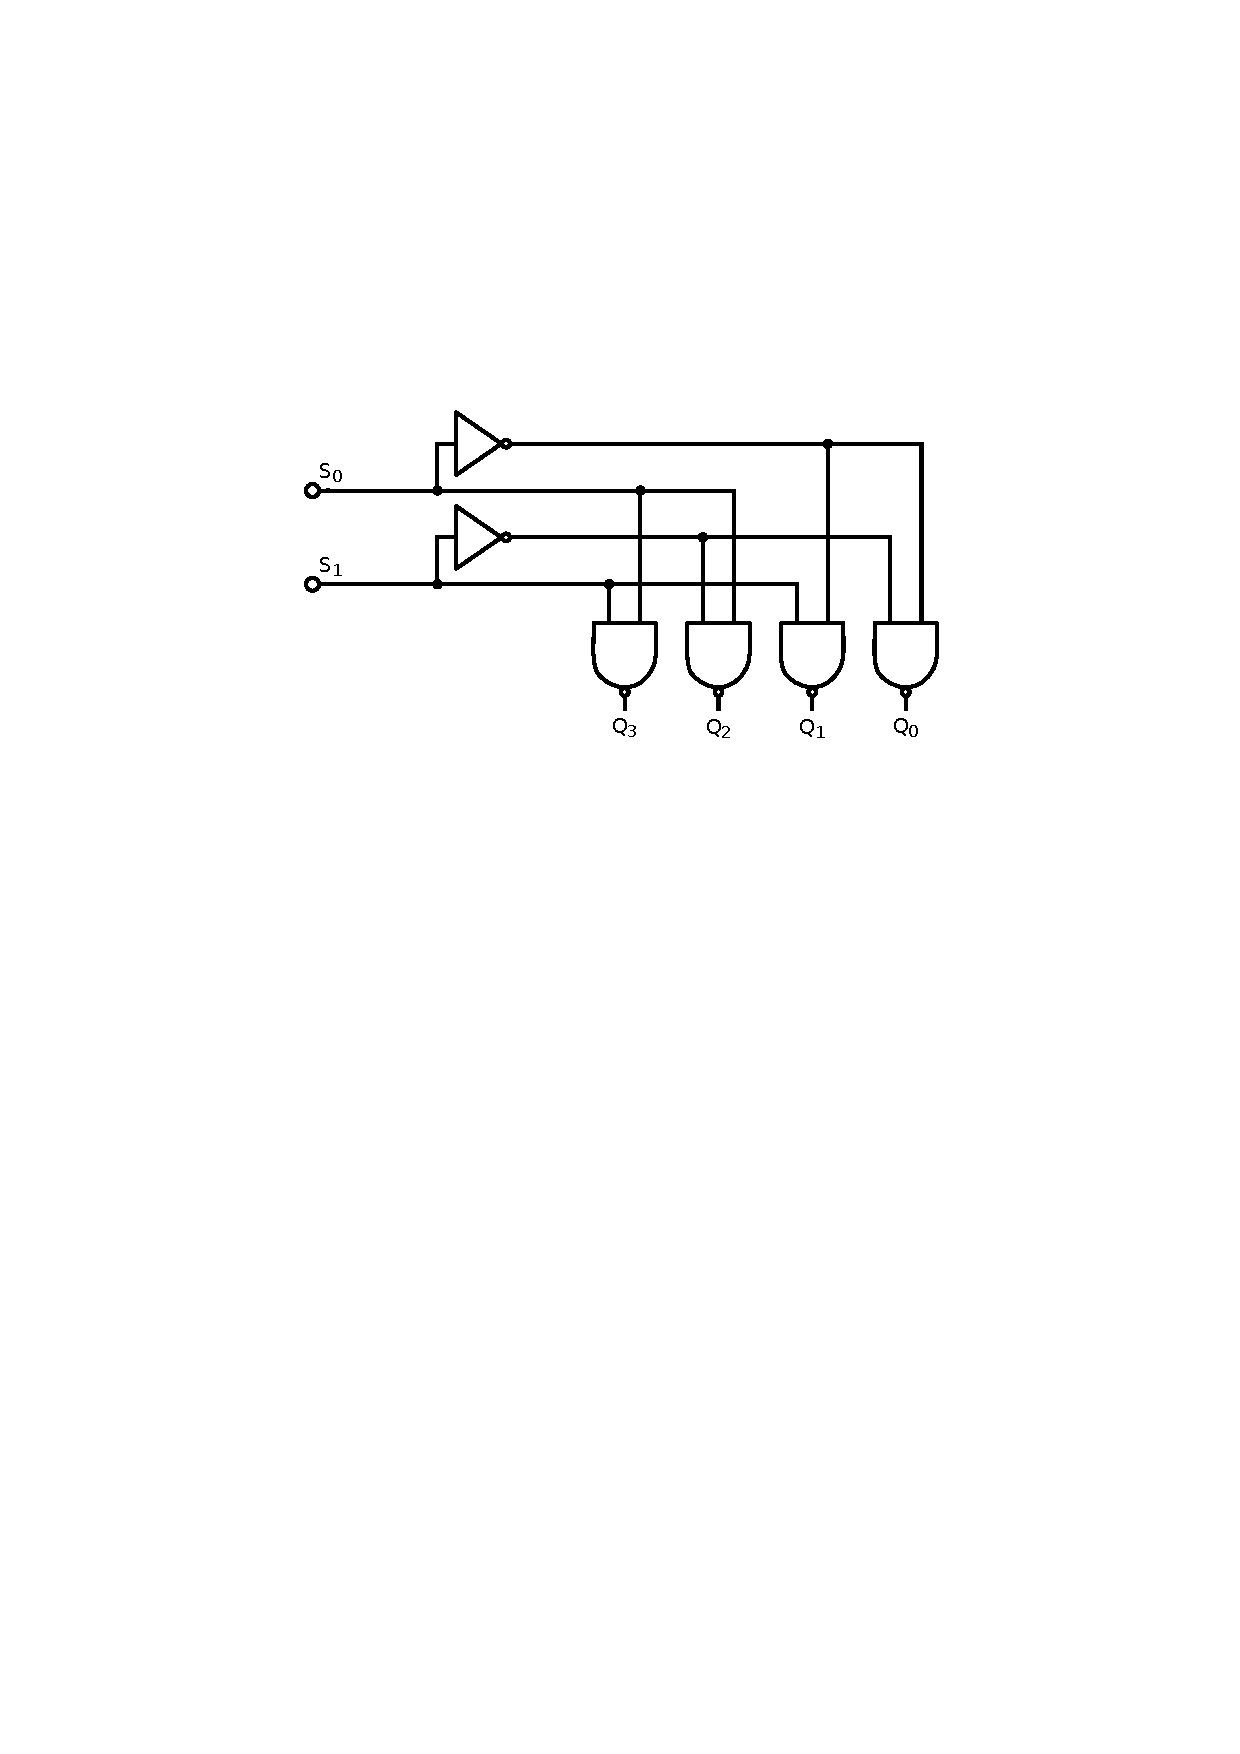
\includegraphics[width=.35\textwidth]{../E10/latex/selector.pdf}
\caption{.}
\label{cir10:selector}
\end{wrapfigure}

Per permettere la selezione del segnale abbiamo bisogno di implementare la seguente tabella di verità (con $S_0$ ed $S_1$ i segnali di selezione che passeranno sui due cavi di selezione).

\begin{table}[htpc]
\centering
{\renewcommand{\arraystretch}{1.1}%
\begin{tabular}{|c|c|c|c|c|c|}
\hline
$S_0$ & $S_1$ & $Q_0$ & $Q_1$ & $Q_2$ & $Q_3$ \\
\hline
0 & 0 & 0 & 1 & 1 & 1\\
\hline
0 & 1 & 1 & 0 & 1 & 1\\
\hline
1 & 0 & 1 & 1 & 0 & 1\\
\hline
1 & 1 & 1 & 1 & 1 & 0\\
\hline
\end{tabular}}
\label{tab10:multiplx_selezione}
\end{table}

\begin{wraptable}[9]{c}{.3\textwidth}
\centering
{\renewcommand{\arraystretch}{1}%
\begin{tabular}{|c|c|c|}
\hline
\diaghead{\theadfont lololololo a} {$S_0$}{$S_1$}& 0 & 1\\
\hline
0 & 0 & 1\\
\hline
1 & 1 & 1\\
\hline
\end{tabular}}
\caption{}
\label{tab10:multiplex_selezione_Q}
\end{wraptable}

In questo modo in uscita avremo come 0 solo la $Q_i$ relativa al segnale selezionato con i due segnali di selezione.

Per far ciò, possiamo dividere il problema come se ogni $Q_i$ abbia una mappa di Karnaugh associata come in Tabella \ref{tab10:multiplex_selezione_Q}.\footnote{Lo svolgiamo per $Q_0$ ma gli altri tre casi sono analoghi}

Otteniamo dunque, considerando per ogni mappa lo 0 come stato logico che ci interessa
$$Q_0 = \overline S_0 \overline S_1 \quad Q_1 = S_0 \overline S_1 \quad Q_0 = \overline S_0 S_1 \quad Q_3 = S_0  S_1$$

E' dunque facile vedere che una implementazione di questo sistema è il circuito logico in Figura \ref{cir10:selettore}.

\subsubsection{Multiplexing}


\begin{wrapfigure}[12]{l}{0.45\textwidth}
\centering
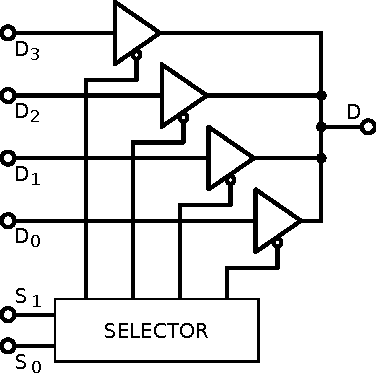
\includegraphics[width=.25\textwidth]{../E10/latex/mult.pdf}
\caption{.}
\label{cir10:mult}
\end{wrapfigure}

Dati i segnali $Q_i$ del circuito di selezione, ora dobbiamo implementare un circuito che passi al cavo di trasmissione solo il segnale che ci interessa. Possiamo dunque utilizzare delle porte tri-state con ingresso di attivazione negato; infatti, collegando a questo ingresso uno dei segnali $Q_i$, faremo passare il segnale $D_i$ (collegato all'altro ingresso della tri-state) se e solo se $Q_i=0$. Un altro vantaggio di utilizzare le tri-state è quello di avere un'alta impedenza quando $Q_i$ sia ad 1 logico (e dunque il segnale selezionato è un altro), evitando cortocircuiti alle uscite delle tri-state (sono tutte collegate al cavo di trasmissione).

Il circuito di multiplexing è in Figura \ref{cir10:multiplex}.

\subsubsection{De-multiplexing}

\begin{wrapfigure}[10]{l}{0.45\textwidth}
\centering
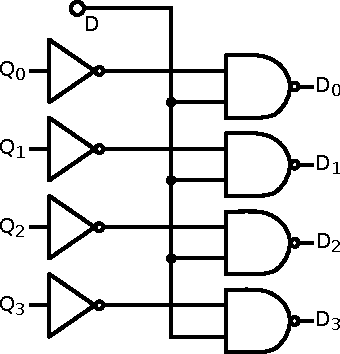
\includegraphics[width=.25\textwidth]{../E10/latex/demult.pdf}
\caption{.}
\label{cir10:demult}
\end{wrapfigure}

Portando i segnali $S_0$ ed $S_1$ di chi invia il segnale ad un selettore (uguale al precedente), il ricevente può costruire un circuito che passi in uscita il dato inviato.

Per far ciò, dobbiamo innanzitutto negare i segnali $Q_i$ (si veda tabella del selettore) per poi inviarli separatamente ad una porta AND: considerandola come un interruttore, e collegando le altre entrate al cavo di trasmissione, avremo in uscita dedicata solo il dato richiesto, e sugli altri lo 0 logico. Il circuito di de-multiplexing è in Figura \ref{cir10:de-multiplex}.
